Sections~\ref{sec:feature_salience}~and~\ref{sec:deep_learning_salience}
have focused on identifying the most important content for summary inclusion,
while punting somewhat on summary generation -- extractive summarization 
minimizes significantly the burden of creating fluent text. 
Abstractive text generation adds significant challenges to summary creation, 
but its benefits are many: the ability to achieve tighter compression ratios
for space constrained scenarios \citep{fan2017controllable}, the potential
to target different reading levels \citep{margarido2008automatic}
or style \citep{shen2017style}, and more pragmatically, in
an increasingly copy-protected web, abstractive generation may be the only 
legally viable option for content aggregation services 
\citep{kassam2014google}.

With this expressive power comes the danger that the generated text may
misrepresent or misconstrue the source material. Trust in machine learning
models is increasingly being recognized as an important factor in user 
adoption \citep{ribeiro2016should}, and mistakes of this kind will be extremely
important for users relying summarization to make high stakes decisions.

\begin{figure}
 \centering
 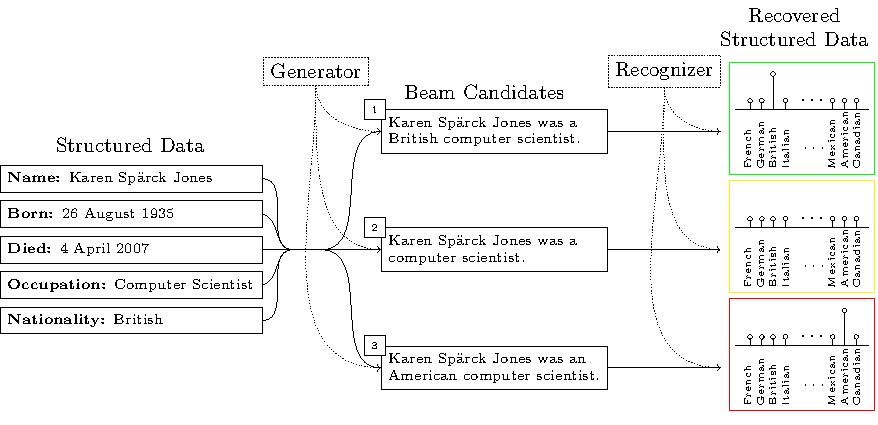
\includegraphics{images/faithful_generation/example1.pdf}
 \caption{Example of faithful generation from structured data. The generator
 is responsible for producing a list (beam) of candidate utterances from the 
 structured data. The recognizer reranks the beam candidates based on the 
 plausibility of the recovered structured data. }
 \label{fig:fgen_example1}
\end{figure}


As a potential solution,
we propose modeling text generation as a two player game between the generator
and recognizer, akin to an auto-encoder \citep{rumelhart1985learning}. 
First, we provide as input to the 
generator some evidence (e.g., raw text or structured data like entries 
from a database). Conditioned on the evidence, the generator must produce 
a list of candidate utterances describing the evidence. The recognizer
reranks the candidates based on the likelihood of predicting the 
correct evidence.
While we will experiment with a variety of loss functions to find something
that works empirically well, we expect in principal to train the generator
to maximize the expected likelihood of evidence under the recognizer.




See \autoref{fig:fgen_example1} for an example 
where we have biographical data (structured data about name, nationality, 
occupation, etc.), and we generate several plausible and implausible 
candidates that are evaluated by the recognizer.
The first candidate is 
 ranked highly because the recognizer can correctly infer that the 
 nationality of Karen Sp\"arck Jones is British (green box). The second 
 candidate is possibly ok because it maximizes entropy over the choice 
 of nationalies (yellow box), i.e. it makes no commitments either way and does
 not produce a non-true statement. The third beam candidate is clearly wrong
 as the recognizer infers that the nationality is American which is a false
 statement according to the true structured data (red box).

In the remainder of this section, we formally define two faithful generation
models, one for generating text from structured data and 
one for generating text from  text data. We conclude by briefly describing some
applications and datasets we will use to evaluate these modls.
